\section{Création du modèle de \glsfmtlong{mt}}
\label{sec.mt-model-creation}

La section précédente fournie une vue de la procédure de création d'un corpus parallèle pour la \gls{mt}.
Dans cette section, nous exploitons ce corpus pour créer et entraîner un modèle de \gls{nmt}.

\subsection{Création du modèle}
\label{subsec.mt-model-creation}

Comme discuté dans Section~\ref{sec.tech}, 
nous avons choisi d'utiliser PyTorch et \foreignlanguage{english}{PyTorch Lightning} pour la partie \gls{dl}.
La classe \verb|Transformer| qui représente notre modèle hérite donc de la classe
\verb|lightning.pytorch.LightningModule| qui elle-même hérite de la classe \verb|torch.nn.Module|.
L'Extrait de code~\ref{code.transformer-init} montre la méthode d'initialisation de cette classe.

\lstinputlisting[
    language=Python,
    caption={Méthode d'initialsation d'un transformeur.},
    label={code.transformer-init},
    firstline=12,
    firstnumber=1
]{assets/scripts/transformer-init.py}

La méthode \verb|__init__| prend en argument les hyperparamètres du modèle
(\verb|d_model|, \verb|nhead|, \verb|num_encoder_layers|, 
\verb|num_decoder_layers|, \verb|dim_feedforward| et \verb|dropout|)
ainsi que des paramètres de configuration de l'entraînement et de l'inférence
(\verb|source_vocab_size|, \verb|target_vocab_size|, \verb|source_pad_idx|, \verb|max_len| et \verb|lr|).

L'appelle à la méthode \verb|super().__init__()| a l'effet de construire par défaut un \verb|LightningModule|.
Les lignes qui suivent cette instruction permettent d'initialiser ce module 
en définissant les couches qui le composent.
Parmi ces couches, la plus importante et \verb|self.transformer|,
un objet de la classe \verb|nn.Transformer|.
Tous les autres modules sont des couches de prétraitement (encodage positionnel)
ou de post-traitement (projection linéaire).
La Figure~\ref{fig.arch} montre le graphe de calcul du modèle résultant.

\begin{table}[hbt]
    \begin{center}
        \begin{tabular}{|l|l|l|l|}
            \cline{2-4}
            \multicolumn{1}{c|}{}& \verb|Name|& \verb|Type|         & \verb|Params|                     \\
            \hline
            0                    & \verb|input_embedding|           & \verb|Embedding|          & 320 K \\
            \hline
            1                    & \verb|input_position_embedding|  & \verb|Embedding|          & 6.4 K \\
            \hline
            2                    & \verb|output_embedding|          & \verb|Embedding|          & 320 K \\
            \hline
            3                    & \verb|output_position_embedding| & \verb|Embedding|          & 6.4 K \\
            \hline
            4                    & \verb|transformer|               & \verb|Transformer|        & 201 K \\
            \hline
            5                    & \verb|transformer.encoder|       & \verb|TransformerEncoder| & 75.8 K\\
            \hline
            6                    & \verb|transformer.decoder|       & \verb|TransformerDecoder| & 126 K \\
            \hline
            7                    & \verb|linear|                    & \verb|Linear|             & 325 K \\
            \hline
            8                    & \verb|dropout|                   & \verb|Dropout|            & 0     \\
            \hline
        \end{tabular}
        \ \\[.5cm]
        \begin{tabular}{ll}
            1.2 M & Paramètres entraînables       \\
            0     & Paramètres non entraînables   \\
            1.2 M & Paramètres totaux             \\
            4.719 & Taille totale estimée (en Mo) \\
        \end{tabular}
    \end{center}
    \caption{Résumé du modèle.}
    \label{tab.model-summary}
\end{table}

En utilisant les valeurs proposées dans le Chapitre~\ref{chap.conception} pour les hyperparamètres :
\[
    \begin{array}{l}
        d_{\mathrm{model}} = d_{\mathrm{FFN}} = 64\\ 
        N_{\mathrm{head}} = 4\\ 
        N_{\mathrm{encoder}} = N_{\mathrm{decoder}} = 3
    \end{array}
\]
nous obtenons un modèle dont la Table~\ref{tab.model-summary} résume les paramètres par couche.

\begin{figure}[htb]
    \begin{center}
        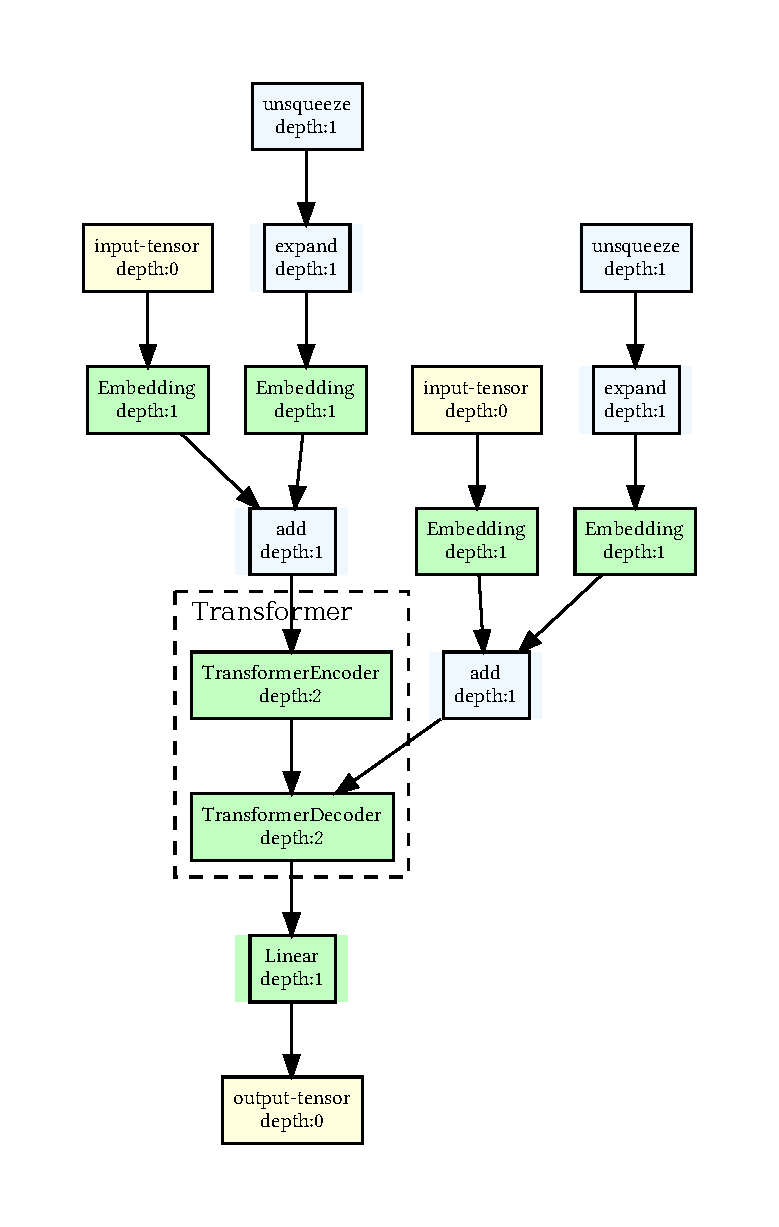
\includegraphics[width=.6\textwidth]{assets/pdf/arch.pdf}
    \end{center}
    \cprotect\caption[Graphe de calcul du modèle définit dans la classe \verb|Transformer|]%
    {Graphe de calcul du modèle définit dans la classe \verb|Transformer| \((\text{profondeur} = 2).\)}
    \label{fig.arch}
\end{figure}

\subsection{Entraînement}
\label{subsec-mt-training}

Pour entraîner le modèle,
un objet \emph{entraîneur} de la classe \verb|lightning.pytorch.Trainer| est utilisé.
Pour configurer sans comportement, plusieurs paramètres sont utilisés (voir Extrait de code~\ref{code.trainer}
\begin{itemize}
    \item \verb|max_epochs| : le nombre maximal des passes sur le corpus d'entraînement.
    \item \verb|deterministic| : un indicateur booléen, s'il est mis à \verb|vrai|, 
    des algorithmes déterministes sont utilisés pour la reproductibilité.
    \item \verb|logger| : le journaliseur à utiliser pour garder trace des métriques.
    \verb|WandbLogger| utilise \emph{\foreignlanguage{english}{Weights \& Biases}} pour la journalisation.
    \item \verb|callbacks| : une liste de rappels de fonctions à effectuer à la fin de chaque époque.
    \verb|early_stopping| implémente l'arrêt précoce et \verb|checkpoint| permet de sauvegarder le meilleur modèle.
    \item \verb|gradient_clip_val| : un majorant sur la norme du vecteur gradient.
    Son but est d'éviter l'explosion des gradients.
\end{itemize}
Pour lancer l'entraînement, il suffit d'appeler la méthode \verb|fit| de l'entraîneur comme suit :
\lstinline[language=Python]|trainer.fit(model, datamodule=dm)|.

\begin{lstlisting}[
    language = Python,
    caption  = {Creation de l'entraîneur.},
    label    = {code.trainer}
]
trainer = Trainer(
    max_epochs=epochs,
    deterministic=True,
    logger=WandbLogger(project="unaphasiator")
    callbacks=[early_stopping, checkpoint],
    gradient_clip_val=1.0,
)
\end{lstlisting}

Le paramètre \verb|datamodule| passé à la méthode \verb|Trainer.fit| est un objet de classe
\verb|lightning.pytorch.LightningDataModule|.
Il s'agit d'une classe d'utilité qui implémente des fonctions de chargement de données.
Ses 3 méthodes \verb|train_dataloader|, \verb|val_dataloader| et \verb|test_dataloader|
retournent respectivement les chargeurs d'entraînement, de validation et de test.
L'entraîneur se charge de les appeler au moment opportun.

\subsection{Réglage des hyperparamètres}%
\label{subsec.hparam-tuning}

Pour cette tâche, nous avons utilisé \emph{\foreignlanguage{english}{Sweeps}},
un outil fourni par \foreignlanguage{english}{Weights \& Biases}.
Pour l'utiliser, il faut créer une configuration qui définit l'espace et la stratégie de recherche pour les hyperparamètres.
Trois stratégies de recherche sont offertes :

\begin{itemize}
    \item \foreignlanguage{english}{Grid} : une recherche exhaustive sur l'espace des possibilités.
    Cette méthode garantie l'optimalité du résultat, mais elle est trop coûteuse 
    et ne marche qu'avec un espace de recherche fini.
    \item \foreignlanguage{english}{Random} : une recherche aléatoire sur l'espace de possibilité.
    Cette méthode ne donne pas de garanties sur la qualité des hyperparamètres qu'elle produit.
    Cependant, elle est beaucoup plus rapide que la recherche exhaustive 
    (car il est possible de définir le nombre des combinaisons à explorer)
    et elle peut être utilisée sur un espace infini.
    \item \foreignlanguage{english}{Bayesian} : une méthode d'amélioration itérative.
    Sa première itération est identique à la recherche aléatoire,
    mais après elle utilise l'information sur le dernier essai pour informer les choix des paramètres du suivant.
    Elle converge généralement vers la solution optimale.
\end{itemize}

Pour définir l'espace de recherche, un dictionnaire ou un fichier \verb|yaml| est utilisé.
L'objet de configuration possède 3 clés obligatoires :

\begin{itemize}
    \item \verb|methode| : la stratégie de recherche.
    \item \verb|metric| : la métrique à optimiser. Il faut fournir le nom de la métrique, le mode d'optimisation
    (\verb|maximize| ou \verb|minimize|) et éventuellement une cible à atteindre.
    \item \verb|parameters| : un dictionnaire qui contient la définition de l'espace des paramètres.
    Chaque paramètre est défini par un couple clé-valeur.
    La clé est le nom du paramètre et la valeur est un dictionnaire qui contient les informations suivantes :
    \begin{itemize}
        \item Si la valeur du paramètre est fixée, il suffit de fournir sa valeur pour la clé \verb|value|.
        \item Si le paramètre a un nombre fini de valeurs possibles, il faut fournir la liste de ces valeurs
        pour la clé \verb|values| et éventuellement sa loi de probabilité pour la clé \verb|probabilities|.
        Si cette dernière n'est pas fournie, la loi uniforme est utilisée.
        \item Si le paramètre est continu, il faut fournir une loi de probabilité pour la clé \verb|distribution|
        en donnant le nom de la loi et ses paramètres.
    \end{itemize}
\end{itemize}

Ci-dessous un exemple de configuration pour une recherche bayésienne.
La métrique à maximiser est \verb|val/bleu_score| et sa valeur cible et de 99.
Les paramètres \verb|lr| et \verb|dropout| sont continus et suivent une loi log-uniforme
sur les intervalles \([10^{-5}, 10^{-1}]\) et \([0.1, 0.5]\) respectivement.
Le paramètre \verb|batch_size| est fixé à 256.

\begin{verbatim}
method: bayes
metric:
  name: val/bleu_score
  goal: maximize
  target: 99
parameters:
  lr:
    distribution: log_uniform_values
    min: 1.e-5
    max: 1.e-1
  dropout:
    distribution: log_uniform_values
    min: 0.1
    max: 0.5
  batch_size:
    value: 256
\end{verbatim}

Une fois la configuration définie, 
il suffit de créer une \foreignlanguage{english}{Sweep} en appelant la méthode \verb|wandb.sweep|,
puis de lancer la recherche en appelant la méthode \verb|wandb.agent|.
Cette méthode prend en paramètre l'identifiant de la \foreignlanguage{english}{Sweep}, 
une fonction qui définit l'entraînement et le nombre d'essais à effectuer (voir Extrait de code~\ref{code.sweep}).

\begin{lstlisting}[
    language=Python,
    caption={Création et lancement d'une \foreignlanguage{english}{Sweep}.},
    label={code.sweep}
]
with open("config/sweep.yaml") as cfg:
    sweep_cfg = load(cfg, Loader)

sweep_id = wandb.sweep(sweep_cfg, project="unaphasiator")
wandb.agent(sweep_id, train, count=10)
\end{lstlisting}



